\documentclass[preview,border=5pt]{standalone}
\usepackage{teaching}
\definecolor{slightblue}{RGB}{245,248,255}
\begin{document}
\pagecolor{slightblue}


\centering

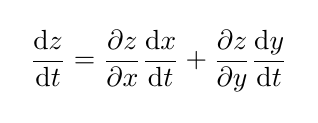
\begin{tikzpicture}[yscale=2,xscale=1,scale=0.5,inner sep=0.3mm, label distance=1.5mm]

\node(t) at (0,1) {$\displaystyle\frac{\mathrm{d}z}{\mathrm{d}t} = \frac{\partial z}{\partial x}\frac{\mathrm{d}x}{\mathrm{d}t} + \frac{\partial z}{\partial y}\frac{\mathrm{d}y}{\mathrm{d}t}$};

\end{tikzpicture}

\end{document}